\section{Introduction}
\label{sec:intro}

\begin{figure*}[!t]
\centering
% Generated by scripts/figura1_drawio.py (numbers: scripts/numeros_fig1.csv;
% thumbnails: scripts/figura1_insumos.py); editable source figures/fig1_overview.drawio.
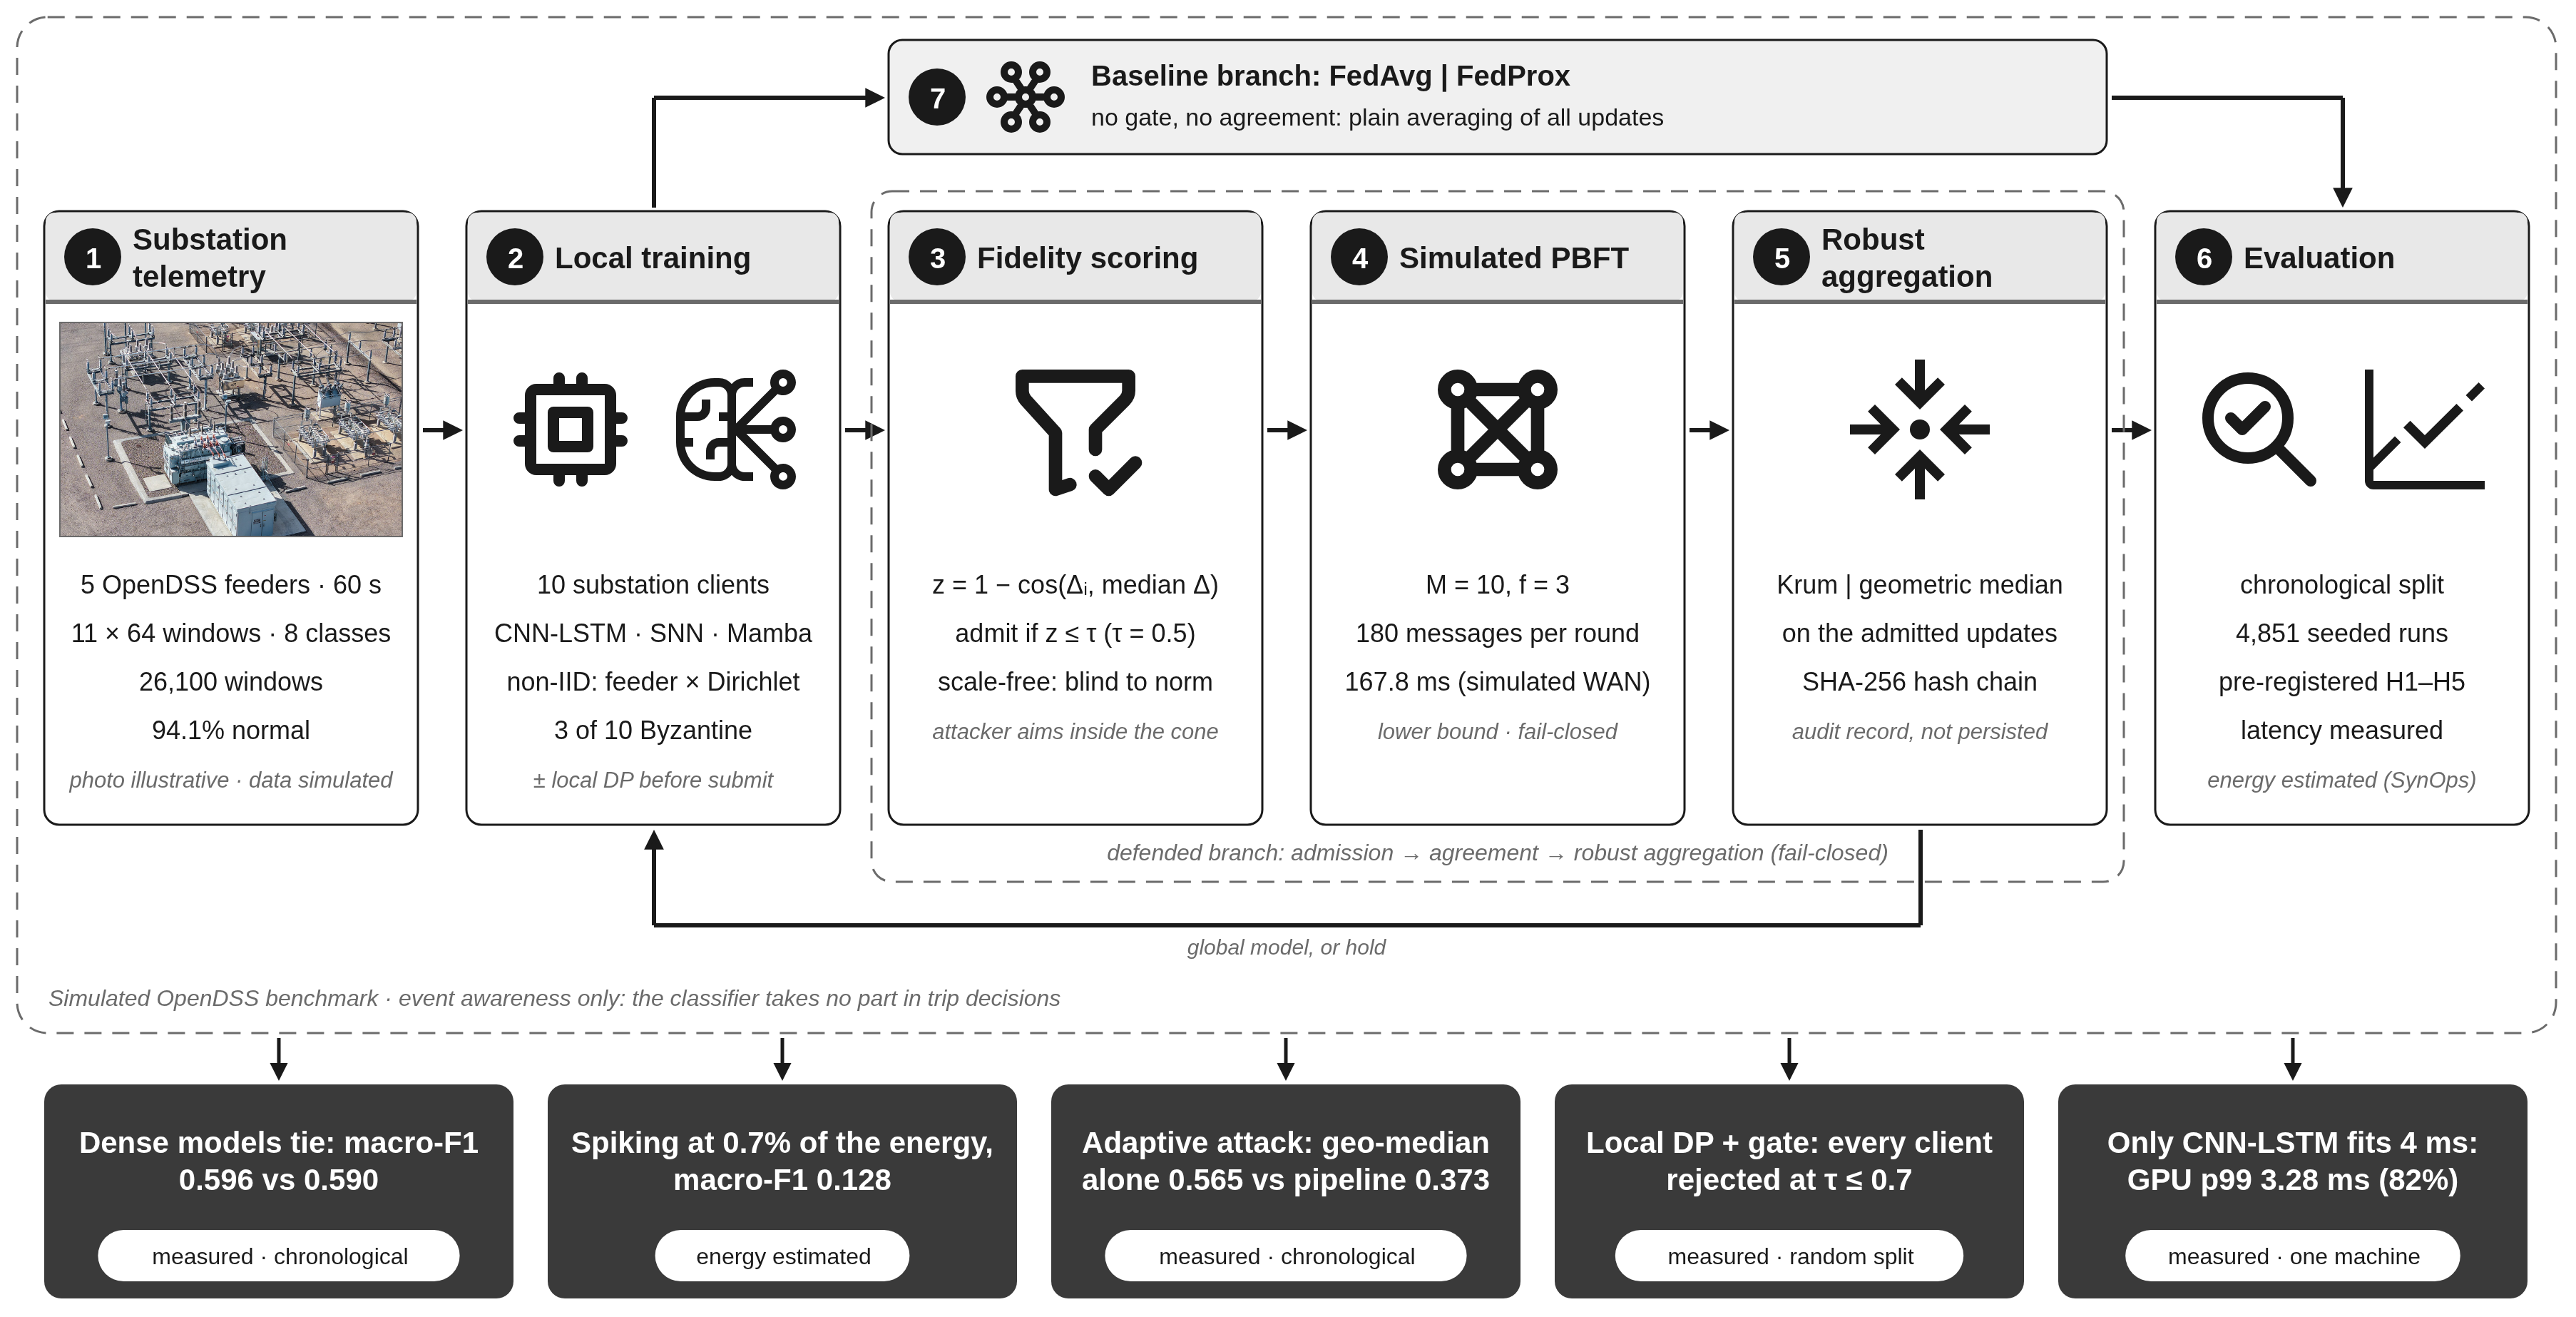
\includegraphics[width=\textwidth]{figures/fig1_overview.png}
\caption{\sysname{} overview: substation telemetry (1) through local
training (2), fidelity scoring (3), simulated PBFT (4) and robust
aggregation (5) to evaluation (6), against the FedAvg/FedProx baseline (7);
bottom, headline results with evidence tags. Photo illustrative (CC0).}
\label{fig:pipeline}
\end{figure*}

Substation gateways conforming to the IEC 61850 family publish
time-aligned electrical measurements -- per-phase voltages and currents,
power, zero-sequence quantities, frequency -- that carry the signature of
the events an operator cares about: ground faults, phase-to-phase faults,
cold-load pickup, sustained sags and swells. Classifying those events
\emph{at the substation edge} shortens the path from measurement to
situational awareness: it feeds control-room triage, inspection
scheduling and reliability analytics. It is an \emph{event-awareness}
function, not a protection function -- the classifier labels windows in a
telemetry stream and takes no part in any trip decision. At the 60\,s
cadence this telemetry delivers, one $T{=}64$ window spans about an hour
of acquisition, which fixes the timescale everything here operates on.

Four constraints make the target hard, and they are usually studied one
at a time. \emph{Data cannot be pooled}: no single distribution utility
holds enough labelled events to train a deep classifier, and pooling
across utilities collides with confidentiality and
critical-infrastructure rules -- the natural fit is cross-silo federated
learning \cite{mcmahan2017}, a few institutional participants with
substantial local data and no willingness to release it. \emph{The
federation is non-identically distributed by construction}: substations
sit on different feeders with different load mixes, generation
penetration and event populations, so heterogeneity is the physical
situation, not a nuisance parameter. \emph{The edge is energy- and
latency-bounded}: devices are fanless and retrofit-powered, the stream is
overwhelmingly normal operation -- the regime an event-driven spiking
classifier should exploit \cite{eshraghian2023,horowitz2014} -- and a
classifier co-resident with protection-adjacent signalling must fit
inside the 4\,ms fast-message transfer-time yardstick the
intrusion-detection literature already uses
\cite{ustun2021,moore2026}. \emph{The federation is adversarially
exposed}: a compromised gateway is a Byzantine participant, a
sophisticated one knows the defense it faces \cite{fang2020,shejwalkar2021},
there is no trusted server-held clean dataset \cite{cao2021fltrust}, and
the local-differential-privacy mechanism that makes participation
acceptable makes honest clients look like attackers
\cite{guerraoui2021podc}.

This paper presents \sysname, a framework that handles all four
constraints in one system, together with the physics-based benchmark
generator that produces its data (Figure~\ref{fig:pipeline} draws the
end-to-end path). \sysname{} is a research artifact: the
simulation, federated engine, attack suite, validation pipeline,
experiment runner and analysis code are released together, and the
batteries behind Section~\ref{sec:results} regenerate from committed
manifests, with per-run configuration hashes verifying canonically for
$67\%$ of the original battery's records.

\subsection{Contributions}
\label{sec:contributions}

\begin{enumerate}\setlength{\itemsep}{1pt}
\item \textbf{A reproducible, physics-grounded federated benchmark
  generator} (Section~\ref{sec:testbed}). Five standard feeders solved
  in quasi-static time series with sample-accurate event injection, a
  modelled measurement chain and a realistic rare-event prior; the
  federation is non-IID on two axes -- feeder identity and Dirichlet
  label skew \cite{hsu2019}. We claim the generator, not the task
  \cite{husnoo2023fedisa,husnoo2023feddisc,li2025fdia}.
\item \textbf{A three-architecture edge comparison under robust
  federation} (Sections~\ref{sec:arch}, \ref{sec:results}). A
  convolutional--recurrent reference, a surrogate-gradient spiking
  network and a selective state-space (Mamba) model on the same
  benchmark and admission pipeline -- a federated spiking classifier on
  substation measurements, and a state-space model in this setting, have
  no precedent \cite{venkatesha2021,nguyen2025robust,mahapatra2021}. The
  honest finding is a trade-off on the leakage-controlled split: the two
  dense models tie, the spiking model is two orders of magnitude cheaper
  in energy but collapses, and only the reference fits a co-resident
  4\,ms envelope.
\item \textbf{A defense-aware attacker carried end-to-end}
  (Section~\ref{sec:threat}). An adversary that knows the admission rule
  constructs in closed form an update inside the admissible cone, plus a
  separate magnitude lever exploiting the scale-freeness of cosine
  scoring \cite{fang2020,shejwalkar2021,baruch2019,xie2019}, evaluated
  against both robust aggregators with the evasion-versus-damage
  asymmetry measured.
\item \textbf{Consensus overhead measured next to the accuracy it buys}
  (Sections~\ref{sec:arch}, \ref{sec:results}). Exact message counts and
  simulated wide-area latency per round, plus the ablation the
  agreement-plus-aggregation literature \cite{kfc2025,li2024brfl}
  usually omits: the pipeline against the robust aggregator standing
  alone. Agreement buys auditability, not accuracy.
\item \textbf{An empirical privacy-versus-admission account}
  (Section~\ref{sec:results}). That differential privacy composes poorly
  with Byzantine resilience is a theorem, and not ours
  \cite{guerraoui2021podc}; we provide the
  measured account of honest false-rejection against attacker admission
  across noise multiplier and threshold, annotated with the R\'enyi
  privacy budget \cite{mironov2017}. At every usable privacy level the
  gate fails closed: the mechanisms are incompatible, not tunable.
\item \textbf{A compute-share budget for waveform-window classifiers}
  (Section~\ref{sec:results}). Measured latency percentiles for all
  three models against the 4\,ms fast-message envelope -- the adjacent
  literature benchmarks packet-level detectors against that figure
  \cite{ustun2021,moore2026}; waveform classifiers have not been placed
  in it before.
\end{enumerate}

\subsection{What this paper does not claim}
\label{sec:nonclaims}

Stating the boundary is cheaper than being corrected at it. We do not
claim first federated learning for power-system fault classification
\cite{husnoo2023fedisa,husnoo2023feddisc}, the discovery of the
privacy--robustness tension \cite{guerraoui2021podc}, or novelty in
combining Byzantine agreement with robust aggregation
\cite{kfc2025,li2024brfl}. We do not claim a hardware energy measurement
(figures are SynOps estimates \cite{horowitz2014}, arithmetic only),
field validation (data come from a simulator;
Section~\ref{sec:limitations}), or end-to-end verification of the
hash-chained ledger (recomputed by property tests, never persisted). We
do not claim Byzantine-fault-tolerant security under equivocation or
partition (the agreement stage is simulated), a protection function (the
4\,ms figure is a compute-share reference, not a deadline), or that the
spiking classifier beats the reference -- the design target is accuracy
\emph{parity} at lower estimated energy, tested as an equivalence claim.

\subsection{Related work}
\label{sec:related}

Five active lines meet here; each is developed fully, with its most
dangerous neighbour named, in Supplementary Section~\ref{sec:sup-related}
and Table~\ref{tab:positioning}. \emph{Federated grid analytics} is
established \cite{husnoo2023fedisa,husnoo2023feddisc,li2025fdia} -- but
every member consumes a fixed dataset; none constructs the federation
from physics. \emph{Spiking classifiers for power systems} exist on
phasor measurements \cite{mahapatra2021} -- centralized, the strongest
precedent for our energy claim -- and federated spiking learning exists
on vision benchmarks \cite{venkatesha2021,aouedi2023hfedsnn}, recently
under Byzantine attack \cite{nguyen2025robust} but with a non-omniscient
adversary and no consensus layer. \emph{Byzantine-robust
aggregation} is settled \cite{blanchard2017,pillutla2022}; trust
bootstrapping \cite{cao2021fltrust} is excluded (no clean server-side
data exists); defense-aware poisoning defines our adversary
\cite{fang2020,shejwalkar2021,baruch2019,xie2019}.
\emph{Agreement-plus-aggregation} combinations are crowded
\cite{kfc2025,li2024brfl} but report neither the protocol's overhead nor
a defense-aware attacker. \emph{DP--Byzantine composition} is
theoretically understood \cite{guerraoui2021podc} and actively
engineered \cite{gu2024dpbrem}, but no member
of that line supplies a measured operating curve in an application
system. \emph{Latency against the 4\,ms envelope} is standard only for
packet-level intrusion detection \cite{ustun2021,moore2026}. The claim
is not any column of that space but the intersection: no prior system
occupies it.

Formal definitions, the extended related work, the realism parameter
audit, battery and provenance detail, and the complete secondary-results
battery are in the supplementary material.
